\documentclass[english,twoside]{article}

%Various Latex formatting parts are here, to keep master.tex files relatively clean.

%---------------------------------------------------------------------------------------------------
%Things related to fonts and overall page appearance

\usepackage{lmodern}
\usepackage{babel}
\usepackage[T1]{fontenc}
\usepackage[nomarginpar]{geometry}
\geometry{verbose,letterpaper}
\addtolength{\oddsidemargin}{1.0cm} %without these two lines, larger margin is on the OUTSIDE.  We want the larger edge on the INSIDE, to allow room for the three hole punches
\addtolength{\evensidemargin}{-1.0cm}
\setlength\topmargin{0.2in}
\addtolength{\hoffset}{-1.0cm}
\addtolength{\textwidth}{2.0cm}
\addtolength{\voffset}{-1.5cm} %This line is apparently needed on some versions of MikTex XeLatex.  Comment out if your pages appear shifted too high.
\addtolength{\textheight}{3.5cm}
\setlength\headheight{1.25em} %about 12pt for 10-point type; about 14.6pt for 12-point type

\usepackage{fancyhdr}
\pagestyle{fancy}

\newcommand{\headersupplementmark}{} %This can be changed to `Lab' or `Appendix' within master.tex
\fancyhead[LO,RE]{\slshape \rightmark} 
\fancyhead[LE,RO]{\slshape \MakeUppercase{\headersupplementmark}\leftmark}
\usepackage{titlesec} %must be called AFTER fancyhead.
\titleformat{\section}{\normalfont\Large\bfseries}{\headersupplementmark \thesection}{1em}{} % At start of section
\renewcommand{\headersupplementmark}{Lab }

\newcommand\immediateaddcontentsline[3]{%
        \begingroup
        \let\origwrite\write
        \def\write{\immediate\origwrite}%
        \addcontentsline{#1}{#2}{#3}%
        \endgroup
}
\newcounter{tocpartnum}
\renewcommand{\part}[1]{
	\stepcounter{tocpartnum}
	%\phantomsection
	\immediateaddcontentsline{toc}{part}{\Roman{tocpartnum} \hspace{1ex} #1}{}}

\usepackage{tocloft} %Allow us to leave page numbers for Parts out of table of contents
\cftpagenumbersoff{part} %No page numbers for Parts out of table of contents
\renewcommand{\cftsecdotsep}{\cftsubsecdotsep}
\setcounter{tocdepth}{1}
\setlength{\cftbeforesecskip}{10.0pt plus 1.0pt minus 3.0pt} %space between chapter listings in TOC.  Default is 10.0pt plus 1.0pt

\setlength\parskip{\medskipamount}
\setlength\parindent{0pt}

\newcommand{\startappendix}{
	\appendix
	\immediateaddcontentsline{toc}{part}{Appendices} 
		%Doing this instead of \part avoids a Roman number for Appendices in the toc
	\cleardoublepage
	\NoForceSectionOddPage 
		%Makes NO extra page break after each appendix; Appendices can start on odd or even page (right or left side).
	\renewcommand{\headersupplementmark}{Appendix }
	\titleformat{\section}{\normalfont\large\bfseries}{\headersupplementmark \thesection :}{1ex}{}
}

\usepackage{xcolor}
\usepackage[pagecolor={white},nopagecolor={white}]{pagecolor}
\usepackage{microtype} % (apparently not compatible with pdflatex)
%\usepackage{epstopdf} %this package apparently allows pdflatex to work on this document, since all we use are eps figures.
\usepackage{authblk}

\usepackage{hyperref}

%---------------------------------------------------------------------------------------------------
%Footnotes
% Note by MT, 3/19/2017: I have no idea what the code below is actually doing.  
% But the Latex compiler crashes whenI take it out, so for now I'm leaving it in.

%% Special footnote code from the package 'stblftnt.sty'
%% Author: Robin Fairbairns -- Last revised Dec 13 1996
\makeatletter
\let\SF@@footnote\footnote
\def\footnote{\ifx\protect\@typeset@protect
    \expandafter\SF@@footnote
  \else
    \expandafter\SF@gobble@opt
  \fi
}
\expandafter\def\csname SF@gobble@opt \endcsname{\@ifnextchar[%]
  \SF@gobble@twobracket
  \@gobble
}
\edef\SF@gobble@opt{\noexpand\protect
  \expandafter\noexpand\csname SF@gobble@opt \endcsname}
\def\SF@gobble@twobracket[#1]#2{}
\makeatother


%---------------------------------------------------------------------------------------------------
%Things related to sectioning and including files

\usepackage{xr} %used to allow external references, so that master_supplement.tex can reference appendices, for instance.
%\usepackage{newclude} %Allows use of /include*{}
%DANGER DANGER: newclude is NOT compatible with package xr, used for external references.

\usepackage{import}
\usepackage{xparse}
% The following lines define a new command \includelab, for including labs in the master.tex file.
% Usage is \includelab{1}{file} to include it, or \includelab{0}{file} to NOT include it.  
% But all 0's can be overridden by writing \includealllabstrue in the master.tex file, which is easier than deleting 
% fifty individual `%' signs and then remembering to put them all back, which is what you had to do before.
% \includeonly still works as you expect it to.
%
% You can also specify a directory for the file, as in \includelab{1}[path]{file}.
% This provides a clean way to share files between 131, 132, and 125.  For example, within the 132 master file,
% if you want to call a 131 lab, you would use: 
%        \includelab{1}[../../131/StudentGuideModule1/]{velocity/velocity}.  
% Among other benefits, this creates a file velocity/velocity.aux within the 132 directory structure, 
% so that the aux file from 132 does not interfere with the aux file from 131.
\newif\ifincludealllabs

\NewDocumentCommand \includelab { m o m } {%
  \IfNoValueTF  {#2}  {%NO directory {#1} {#2} {#3} \par 
	\ifnum#1=1 \include{#3} 
	\else \ifincludealllabs \include{#3} \fi 
	\fi
	}
  {%There is a directory {#1} {#2} {#3} \par
	\ifnum#1=1 \subincludefrom{#2} {#3} 
	\else \ifincludealllabs \subincludefrom{#2} {#3} \fi 
	\fi
	}
}


%---------------------------------------------------------------------------------------------------
%Packages and new commands providing general utilities

\usepackage{graphicx}
\usepackage{wrapfig}
\usepackage{comment}
\usepackage{makeidx}
\usepackage{esvect}
\usepackage{amsmath} %uncommented by MT 5/2015, used in "E near charged rod"
\usepackage{amssymb}
\usepackage{mathtools} %added by MT 6/2015, for access to dcases environment in finding_v_from_e
% This file loads all packages and makes all definitions used for making various graphs,
% using Tikz and pgfplots.  It was developed in July-August 2019 by Matt Trawick.
% The goal is to pre-define several basic types of graphs used in our manuals (plain axes
% with qualitative graphs, or empty grids with scales, etc.) that could be easily used and
% tweaked throughout the manual, for stylistic uniformity.
% These could gradually (or not so gradually) replace the hodge-podge of .eps files
% generated from difference sources that are currently used in the manuals.
\usepackage{pgfplots}
\usepackage{sansmath} 
\usepgfplotslibrary{groupplots}
\usetikzlibrary{pgfplots.groupplots}
\usetikzlibrary{math}
\usepackage{xparse} %used for \NewDocumentCommand
% xparse is actually used elsewhere as well, so doesn't need to be called here for the main lab manual.
% I'm keeping the line in for when this file is called by another .tex file, for instance if you're just testing
% how things work.

\pgfplotsset{compat=1.16} %Version 1.16 is the current version, as of July 2019

%-------------------------------------------------------------------------
% Below, set several style choices used throughout the manual.
\tikzset{every picture/.style={font=\sffamily}}

\pgfplotsset{
  tick label style = {font=\sansmath\sffamily},
%  every axis label = {font=\sansmath\sffamily},
%  legend style = {font=\sffamily},
%  label style = {font=\sffamily}
	samples = 200,
	height = {2in}, width = {2in},
	every axis/.append style={line width=0.8pt}, %default appears to be about 0.4pt
}


% This pre-defines a "cycle" of colors and styles that can be used for successive plots added to an axis.
% In this case the "cycle" effectively has only one entry, so all plots look the same.
% But note that in order to achieve that effect, I need to repeat the entry, once with a comma, and once
% without a comma.  See the file mwe_cyclelist_weirdness.tex for details.
\pgfplotscreateplotcyclelist{lab_solid}{
	{black, line width = 2pt, mark=none},
	{black, line width = 2pt, mark=none}
	% Note: by my eye, "thick"=0.8 pt, "very thick" = 1.2 pt, "ultra thick" = 1.6 pt
}

%---------------------------------------------------------------------------
% This part predefines several named styles ("lab_noticks_1quad" for a single-quadrant set of blank axes, etc.)
% that can be called for various graphs used throughout the manual.
% Each option within the defined style can be overridden individually as needed, or
% additional options added. For instance,
% 		\begin{lab_axis}[lab_noticks_2quads,
% 			ymin = -0.5,
% 			....
%
% These "styles" are really just lists of options, and can be combined if needed, as in 
% 		\begin{lab_axis}[lab_noticks_2quads,
%			plus_minus_zero_labels
% 			....

% single quadrant:
\pgfplotsset{lab_noticks_1quad/.style={
	cycle list name = lab_solid,
	% every axis plot/.append style={very thick},
	% I now specify thickness in the lab_solid cycle definition, so previous line is not needed.
	every axis plot/.append style={domain=0:0.9*\pgfkeysvalueof{/pgfplots/xmax}},
	axis x line={left, x axis line style={->}}, % solid line with no arrow.
	axis y line={left, y axis line style={->}},
	xmin=0, xmax=1,
	ymin=0, ymax=1, %Although there are no ticks, this seems to be needed to make the ticks disappear.
	tick style={xtick=\empty,ytick=\empty}
}}

% two quadrants (I and IV):
\pgfplotsset{lab_noticks_2quads/.style={
	cycle list name = lab_solid,
	every axis plot/.append style={domain=0:0.9*\pgfkeysvalueof{/pgfplots/xmax}},
	axis x line= {middle, x axis line style={->}}, 
	axis y line= {left,  y axis line style={<->}},
      xlabel style={at=(current axis.right of origin), anchor=west},
	xmin=0, xmax=1,
	ymin=-1, ymax=1, 
	tick style={xtick=\empty,ytick=\empty},
}}

% two quadrants (I and IV), but with labels like for a mathematical function:
\pgfplotsset{lab_noticks_2quads_algebraic/.style={
	cycle list name = lab_solid,
	axis x line= {middle, x axis line style={->}}, 
	axis y line= {left, y axis line style={<->}},
%	xlabel style={at=(current axis.right of origin), anchor=north east},
%	ylabel style={at=(ticklabel* cs:1.0),  rotate=-90, anchor=north east},
algebraic_labels,
	xmin=0, xmax=1,
	ymin=-1, ymax=1, 
	tick style={xtick=\empty,ytick=\empty},
}}

%four quadrants:
\pgfplotsset{lab_noticks_4quads/.style={
	cycle list name = lab_solid,
	every axis plot/.append style={domain=0.85*\pgfkeysvalueof{/pgfplots/xmin} : 
                                                                  0.85*\pgfkeysvalueof{/pgfplots/xmax}  },
	axis x line= {middle, x axis line style={<->}}, 
	axis y line= {middle, y axis line style={<->}},
	xlabel style={at=(current axis.right of origin), anchor=north east},
	ylabel style={at=(ticklabel* cs:1.0), anchor=north east},
	xmin=-1, xmax=1,
	ymin=-1, ymax=1, 
	tick style={xtick=\empty,ytick=\empty},
}}

\pgfplotsset{lab_grid/.style={
	cycle list name = lab_solid,
	% every axis plot/.append style={ultra thick},
	% Interestingly, previous line does NOT override thickness in lab_solid
%	tick style={grid=both,major tick length=0pt},
	axis line style={draw=none},
	tick style={
		grid=both, 
		major tick length=0pt,
		minor tick length=0pt},
}}

\pgfplotsset{algebraic_labels/.append style={
	xlabel style={at=(current axis.right of origin), anchor=north east},
	ylabel style={at=(ticklabel* cs:1.0), rotate=-90, anchor=north east},
}}

% Use this to add a darker horizontal line at y=0 to lab_grid style graphs.
\pgfplotsset{y0_line/.style={
	extra y ticks={0},
	extra y tick style={
		major grid style=black,
		major tick length=0pt,
		},
}}


% In a groupplot, the y labels can be misaligned if one graph has "longer" tick lables, such as ones that include
% a negative sign.  This command bumps the y label of the current to the left, to match the alignment of the
% y label of the other graph.  To tell it how much to move it over, you need to give it the longest tick label text 
% of the other graph as an argument.  Example: 
% 		ylabel_align={-10}
% Note that it works by actually creating an "extra y tick" on the current graph, but writing the label as
% phantom text that doesn't show up.  For this reason, it will not work with y0_line, because that also works
% by defining an "extra y tick" at zero.
\pgfplotsset{ylabel_align/.style={
	extra y ticks={\pgfkeysvalueof{/pgfplots/xmin}},
	extra y tick labels={\phantom{$#1$}},
 	extra y tick style={
		major tick length=0pt,
		},
}}

% Use this to add y axis labels +, -, and 0 to graphs, presumably to lab_noticks_2quads style graphs.
\pgfplotsset{plus_minus_zero_labels/.style={
	extra y tick style={major tick length=0pt},
	extra y ticks = {-0.8, 0, 0.8},
	extra y tick labels = {\scriptsize{$-$},0,\scriptsize{$+$}},
}}


% The commmand below makes vertical alignment marks through all graphs in a groupplot.
% (Restricted to only a single column, but multiple rows.  The number of rows can be "1" though.)
%
% How to call:
% 		\makegroupverticlas[rows]{x1,x2,x3...}{xmin}{xmax}
% rows is assumed to be 2 if not specified.  xmin and xmax are the min and max values of the axis.
% Oh, and it won't work if you define a name for the group; it must remain the default "group".
%
% This was a giant pain to get to work.  
% The problem seems to be that INSIDE the groupplot environment, tikz knows about xmin and xmax
% (since it can get it from \pgfkeysvalueof{/pgfplots/xmin} ) but does not know about the top and bottom
% of the whole group; only of a single axis.
% But OUTSIDE the grouplot environment, tikz knows about the top and bottom of the group
% (from group c1r1.north west, for instance), but does not know about the scale of the x axis.
% Or at least I couldn't figure out how to get it to know about the x axis.  Maybe someone else can.
% If so, it would be a nice improvement to NOT have to pass it xmin and xmax, or even the number of
% rows, for that matter. 
\NewDocumentCommand \makegroupverticals {o m m m} {
	\coordinate (TL) at (group c1r1.north west); % top left
      \IfNoValueTF  {#2} {%If no lastrow given, assume two rows
		\coordinate (BR) at (group c1r3.south east); % bottom right
		}
	{ % else use the value for the number of the last row
		\coordinate (BR) at (group c1r#1.south east); % bottom right
		}
	\newdimen\xleft
	\pgfextractx\xleft{\pgfpointanchor{TL}{center}}
	\newdimen\xright
	\pgfextractx\xright{\pgfpointanchor{BR}{center}}

	\newdimen\xx
	\foreach \x in {#2} { 
		\tikzmath{\xx = \xleft + (\xright - \xleft) * ((\x - #3) / (#4 - #3))  ;}
		\draw[black, thick, dashed] (\xx, |- TL) -- (\xx, |- BR);
		}
}

% Here's an older version of makegroupverticals.
% It does not work, because the x axis coordinates in \x are often wrong,
% Sometimes by a huge amount.  I suspect there's a way to make this work,
% with a small fix, so I'll keep it here.
\NewDocumentCommand \oldmakegroupverticals {o m} {
	\coordinate (toppoint) at  (group c1r1.north);
      \IfNoValueTF  {#2} {%If no lastrow given, assume two rows
		\coordinate (botpoint) at  (group c1r2.south);
		}
	{ % else use the value for the number of the last row
		\coordinate (botpoint) at  (group c1r#1.south);
	}
	\foreach \x in {#2} 
		\draw [black, very thick, dashed] (\x, |- toppoint) -- (\x, |- botpoint);
}


%------------------------------------------------------------------------------------------------------------------
% Finally, this next section defines two (currently) environments, simply for convenience, to make
% these graphs less cumbersome to call.  You can still make graphs by using 
% 		\begin{tikzpicture}
% 		\begin{axis}
%		 .....
% if you want.


% The lab_axis environment, defined below, is basically a thin wrapper around the "tikzpicture" and "axis" 
% environments, combined.  When called in the starred version ("*", see below) it also centers the graph.
% Note that it also puts small vertical spaces above and below the graph.  If this is called multiple times on 
% one line, the vertical spaces will build up and be placed after the graphs, requiring a 
%		\vspace{-2em} 
% (or whatever length you need) to undo.
\NewDocumentEnvironment{lab_axis}{s}{
	\IfBooleanTF #1
		{ \begin{center} } %if starred
		{} %if not starred, do nothing
	\vspace{0em} % Because our lab manual skips lines between paragraphs, we don't need extra space 
	\begin{tikzpicture} 
	\begin{axis}
	}
	{\end{axis} 
	\end{tikzpicture}
	\vspace{0em}
	\IfBooleanTF #1
		{\end{center} } %if starred
		{} %if not starred, do nothing
	 }
% Next four lines allow either 
%	\begin{lab_axis*}... \end{lab_axis*} 
% or 
% 	\begin{lab_axis}*... \end{lab_axis}
\ExplSyntaxOn
\cs_new:cpn {lab_axis*} {\lab_axis*}
\cs_new_eq:cN {endlab_axis*} \endlab_axis
\ExplSyntaxOff

% This new environment is a thin wrapper around the "tikzpicture" and "groupplot" environments, combined.
% When called in the starred version, it is centered as well.  (Here, the "*" goes AFTER the "}", as in
% 		\begin{lab_groupplot}*{}blah blah blah.
% The empty argument above is where you put any line or lines that go after the \end{groupplot} but
% before the \end{tikzpicture}, which would typically be drawing vertical alignment marks
% using \makegroupverticals, or adding other annotations.
\NewDocumentEnvironment{lab_groupplot}{s m}{
	\IfBooleanTF #1
		{ \begin{center} } %if starred
		{} %if not starred, do nothing
	\vspace{0em}
	\begin{tikzpicture}
	\begin{groupplot}
	}
	{\end{groupplot}
	#2
	\end{tikzpicture}
	\vspace{0em}
	\IfBooleanTF #1
		{\end{center} } %if starred
		{} %if not starred, do nothing
	 }



\usepackage{hhline}
\setlength\doublerulesep{0.75pt}
\usepackage{tabularx} %added by MT 6/2015, for fixed width columns, used in rc_circuits
%For fixed width columns:
\newcolumntype{L}[1]{>{\raggedright\arraybackslash}p{#1}}
\newcolumntype{C}[1]{>{\centering\arraybackslash}p{#1}}
\newcolumntype{R}[1]{>{\raggedleft\arraybackslash}p{#1}}
% define a strut for extra vertical space in tables.
\newcommand{\hi}{\rule[-2mm]{0mm}{6mm}}

%I make use of some latex features to manage the section numbers. To use those you have to insert the following lines into the latex preamble (before the %"\begin{document}" command). -gpg
% two new commands to do labelling. - gpg 12/4/13
\newcommand{\customlabel}[2]{%
\protected@write \@auxout {}{\string \newlabel {#1}{{#2}{}}}}

\newcommand{\actlabel}[1]{%
\protected@write \@auxout {}{\string \newlabel {#1}{{\arabic{activity}}{}}}}

\newcounter{activity}

\usepackage{enumitem} %added 3/2016 by MT.  Tested 100% with other labs, looks like it does no harm.
%enumitem package allows enumerate[resume], which allows enumerate to play nicely with wrapfig (see induction1).
%enumitem package also provides very useful [wide] and [nosep] presets. (See, eg. resonance_tubes).
\SetEnumitemKey{labparts}{wide, label=(\emph{\alph*})} %defines labparts to number parts as (a), (b), etc.


\usepackage{chngcntr} %allows control over counters
\counterwithin*{footnote}{section} %resets the footnote counter to 1 at every new section (each lab)
\counterwithin*{equation}{section} %resets the equation counter to 1 at every new section (each lab)
\counterwithin*{figure}{section} %resets the figure counter to 1 at every new section (each lab)

\newcommand\specialcaret {\hspace{0.0ex}\raisebox{0.6ex}{\scalebox{0.7}[0.7]{$\boldsymbol{\wedge}$}}\hspace{0.1ex}}

\newcommand{\makelabheader}
%{Name: \rule{2.0in}{0.1pt}\hfill{}Section: \rule{1.0in}{0.1pt}\hfill{}Date: \rule{1.0in}{0.1pt}}
{Name: \rule{2.0in}{0.1pt}\hfill{}Lab Partner(s): \rule{3.0in}{0.1pt}}


%A new command for putting a box around a paragraph:
\newenvironment{newboxed} %maybe there's a better way to do this.  I just cribbed from the web. --MT
    {\begin{center}
    \begin{tabular}{|p{0.9\textwidth}|}
    \hline\\
    }
    { 
    \\\\\hline
    \end{tabular} 
    \end{center}
    }


%  The following command, \answerspace, should be used to replace \vspace.
%  \vspace{} is not ideal for an answer space for students, for two reasons:
%  1. It can be ignored if it comes at the end of a page, and
%  2. The spacing is exact, and Latex will not stretch or compress it at all to make things fit on a page, which means
%  that other things WILL get stretched or compressed to make things fit, which means those other things will 
%  end up looking bad, and leading to a lot of underfull \vbox warnings.
%  \answerspace fixes both of those problems, specifically allowing the space to grow to up to 1.5 times the stated size.
\newlength\answerlength
\newcommand{\answerspace}[1]{
	\setlength\answerlength{#1}
	\vspace*{1.0\answerlength plus 0.5\answerlength}}

%The following code can be used to make each lab start on odd numbered page (right hand side).
\let\NoExtraPageSection\section
\let\NoExtraPagePart\part
\newcommand{\ForceSectionOddPage}{
	\renewcommand{\section}{\cleardoublepage\NoExtraPageSection}
	\renewcommand{\part}{\cleardoublepage\NoExtraPagePart}
	}
\newcommand{\NoForceSectionOddPage}{
	\renewcommand{\section}{\NoExtraPageSection}
	\renewcommand{\part}{\NoExtraPagePart}
	}


\newif\ifForOneTwentyFive %is set to true in master.tex for PHYS 125.  Allows alternate versions of the labs.  Use with care!

\newcommand{\filename}[1]{{\sffamily\fontshape{sl}\selectfont #1}}
\newcommand{\button}[1]{{\fontshape{sl}\selectfont #1}}

%Next lines implement conditional references, to reference a lab or appendix only if it exists in the document.
\makeatletter
\newcommand{\iflabelexists}[3]{\@ifundefined{r@#1}{#3}{#2}}
%May be slightly tidier to eventually implement this using package etoolbox
%See https://tex.stackexchange.com/questions/111311/how-to-make-a-conditional-reference-to-a-text-label
\makeatother

\hyphenation{im-ped-ance}

 %all general latex packages, commands, and definitions now here.
\newcommand{\coursefolder}{Phys131} %This defines the place students will look for various files
%\ForceSectionOddPage %This option makes each lab start on odd numbered page (right hand side).

%The \includeonly line below is a great way to save time so you don't always have to compile the WHOLE latex document, if for instance you've only made changes to a single lab.  If you want to compile more than two labs, the syntax is \includeonly{lab1,lab2,lab3} with no spaces after the commas.
%The master.pdf produced will have only the title page, TOC, and that single lab, though the other lab names will appear in the TOC.
%\includeonly{rotational_KE/rotational_KE}

%Use the following line to override all of the 1's and 0's in the \includelab statements below
%\includealllabstrue

% to generate the pdf on centos7: latex master;  dvipdfmx master
% to convert images to eps: convert <file>.jpg <file>.pdf; pdftops -eps <file>.pdf

\makeindex
\begin{document}

\newgeometry{total={8in,10.5in},hoffset=0.2in,voffset=0.3in}
%nb: I just messed with the numbers above until it looked okay.  I really don't know what I'm doing. --MT, 4/23/2016
\thispagestyle{empty}
\definecolor{darkblue}{RGB}{0,0,160}
\definecolor{lighterblue}{RGB}{0,128,255} %Looks better on the print shop's printer
\newpagecolor{lighterblue}

\begin{center}
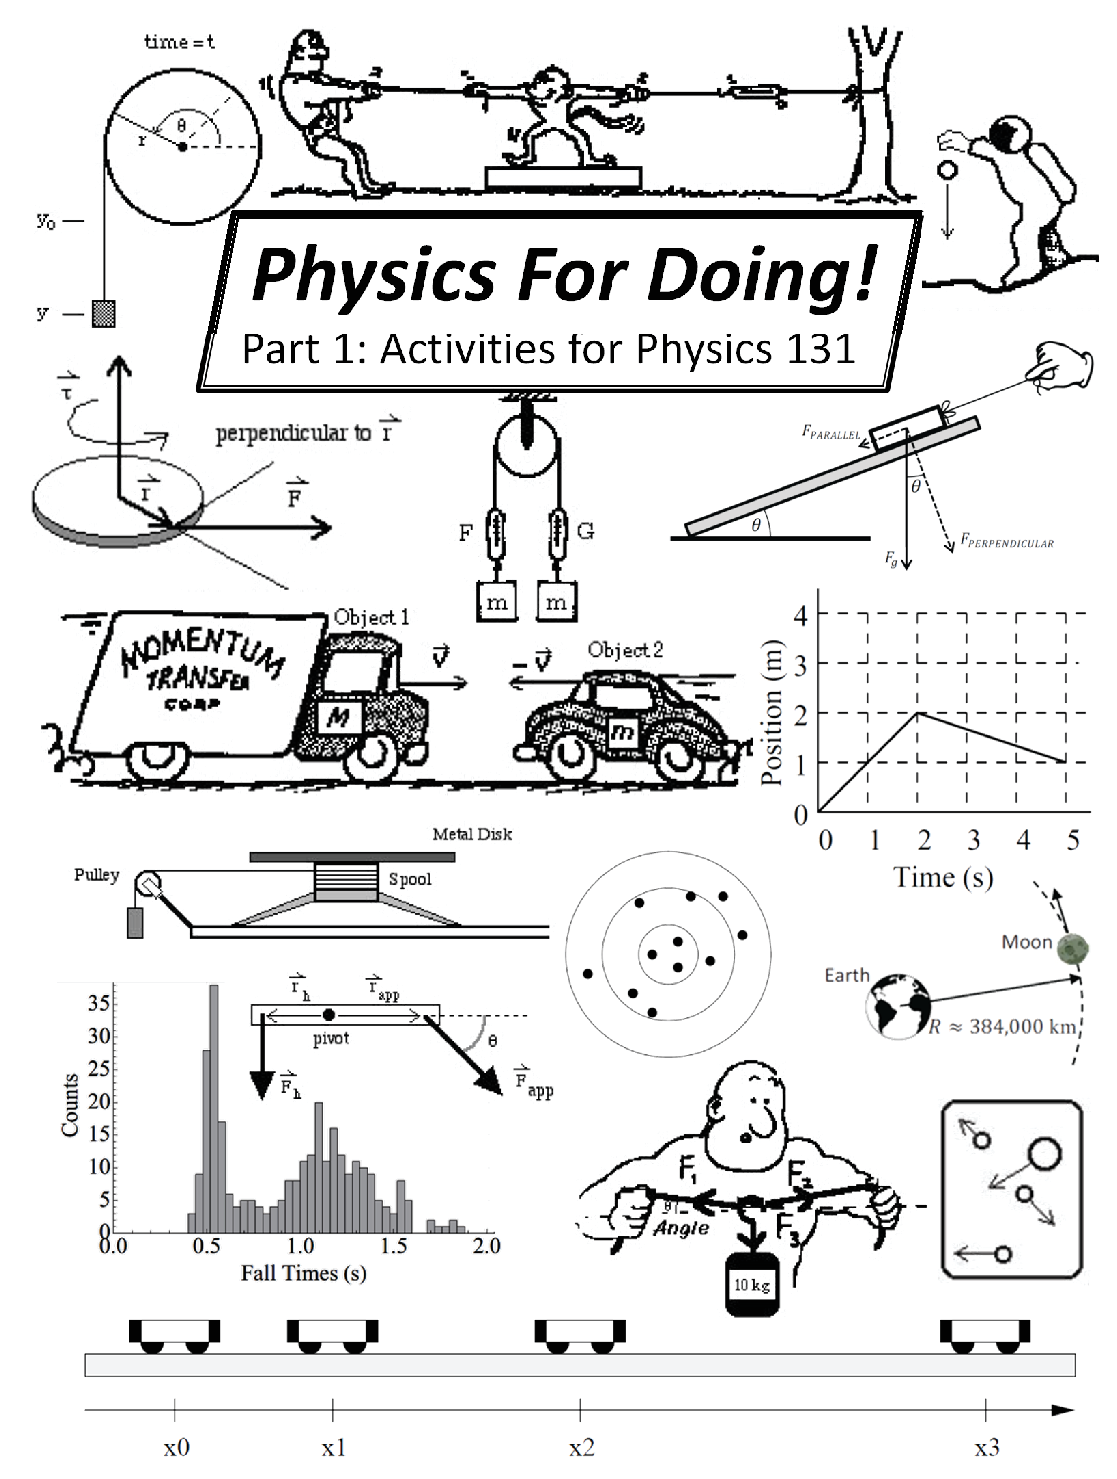
\includegraphics[width=7.3in,trim={0 0 .1cm 0},clip]{131_front_pages/131_front_cover.eps}
\index{color page}
\end{center}
\newpage

\restoregeometry
\restorepagecolor
\thispagestyle{empty}

\
\vfill
\textit{Cover art: Various graphics and diagrams from the activities in this manual.  You'll be doing lots of stuff.}
\pagebreak



\title{Physics For Doing!\\
Part 1: Activities for Physics 131}

\author{Matthew G. Belk}
\author{Emory F. Bunn}
\author{Mirela Fetea\footnote{Current address: Germanna Community College, Fredericksburg, VA}}
\author{Gerard P. Gilfoyle}
\author{Christine C. Helms}
\author{Henry Nebel}
\author{Philip D. Rubin\footnote{Current address: Department of Physics, George Mason University, Fairfax, VA}}
\author{Shaun Serej}
\author{Jack Singal}
\author{Matthew L. Trawick}
\author{Michael F. Vineyard\footnote{Current address: Department of Physics, Union College, Schenectady, NY}}
\affil{Department of Physics, University of Richmond, VA}

\maketitle

\vspace{0.8 in}

%\begin{abstract}

\begin{center}
\large{\textbf{Welcome to Physics 131!}}
\end{center}

The exercises in this manual have been developed to support an investigative
physics course that emphasizes active learning. 
%The units are made up of activities designed to guide your investigations in the laboratory. 
Your written work will consist primarily of documenting
your class activities by filling in the entries in the spaces provided
in the units. The entries consist of observations, derivations, calculations,
and answers to questions. Although you may use the same data and graphs
as your partner(s) and discuss concepts with your classmates, all
entries should reflect your own understanding of the concepts and
the meaning of the data and graphs you are presenting. Thus, each
entry should be written in your own words. It is very important
to your success in this course that your entries reflect a sound understanding
of the phenomena you are observing and analyzing. 

Some of these exercises
have been taken from the Workshop Physics project at Dickinson College
and the Tools for Scientific Thinking project at Tufts University
and modified for use at the University of Richmond. Others have been
developed locally. 
We wish to acknowledge the support we have received for this project
from the University of Richmond and the Instrumentation and Laboratory
Improvement program of the National Science Foundation. 
%\end{abstract}


\newpage
\
\thispagestyle{plain}

\newpage
\
%\setcounter{page}{2} %changed from 1 to 2 on 6/9/15 by MT.  The reason is that in the circuit labs, the odd pages need to be on the right (the fronts of each sheet of paper) and the even pages need to be on the left.  This is critical, because these labs have some pages that are meant to be cut out with scissors, so the backs have to be left blank.  This is done by using the \cleardoublepage command, which requires that the odd/even pages not be reversed from the usual.




\tableofcontents{}
\cleardoublepage

%--------------------------------------------
\part{Kinematics}

\includelab{1}{measuring/measuring}
\includelab{0}{walking_speed/walking_speed}
\includelab{0}{converting_units/converting_units}
\includelab{0}{measurement_length/measurement_length}
\includelab{0}{determining_pi/determining_pi}
\includelab{1}{position/position}
\includelab{1}{velocity/velocity}
\includelab{1}{relating/relating}
\includelab{1}{instantaneous_velocity/instantaneous_velocity}
\includelab{1}{changing/changing}
\includelab{1}{slowing/slowing}
\includelab{1}{equations/equations}
\includelab{0}{measurement/measurement}
\includelab{1}{measurement_uncertainty/measurement_uncertainty}
\includelab{0}{grav_freefall/grav_freefall}
\includelab{1}{acceleration/acceleration}
\includelab{0}{reaction_time/reaction_time}
\includelab{0}{tossed_ball/tossed_ball}
\includelab{0}{independence/independence}
\includelab{0}{ski_jump/ski_jump}
\includelab{0}{projectile/projectile}
\includelab{0}{vectors/vectors}
\includelab{0}{circ_motion/circ_motion}

%--------------------------------------------
\part{Forces}

\includelab{1}{force1/force1}
\includelab{1}{force2/force2}
\includelab{1}{combining/combining}
\includelab{1}{force_mass/force_mass}
\includelab{0}{newton/newton}
\includelab{0}{atwood/atwood}
\includelab{0}{friction/friction}
\includelab{0}{check_your_units/check_your_units}
\includelab{0}{elec_grav/elec_grav}
\includelab{0}{centripetal/centripetal}
\includelab{0}{kepler/kepler}
\includelab{0}{archimedes/archimedes}

%--------------------------------------------
\part{Conservation Laws}

\includelab{0}{work_power/work_power}
\includelab{1}{work_kinetic/work_kinetic}
\includelab{1}{conservation_mech/conservation_mech}
\includelab{0}{eoverm2/eoverm2}
\includelab{0}{conservative/conservative}
\includelab{0}{momentum/momentum}
\includelab{1}{impulse/impulse}
\includelab{0}{newtons_laws/newtons_laws}
\includelab{0}{mom_cons/mom_cons}
\includelab{0}{twod_collisions/twod_collisions}

%--------------------------------------------
%\part{Rotational Motion}

\includelab{0}{ang_lin_displacement/ang_lin_displacement}
\includelab{0}{rotation/rotation}
\includelab{0}{newtons_2law_rot/newtons_2law_rot}
\includelab{0}{rolling/rolling}
\includelab{0}{moment_inertia_feel/moment_inertia_feel}
\includelab{0}{moment_inertia/moment_inertia}
\includelab{0}{rotational_KE/rotational_KE}
\includelab{0}{ang_mom/ang_mom}
\includelab{0}{cons_ang_mom/cons_ang_mom}

%--------------------------------------------
\part{Oscillation}

\includelab{0}{hooke/hooke}
\includelab{1}{periodic_motion/periodic_motion}
\includelab{0}{pendulum_period/pendulum_period}
\includelab{0}{resonance/resonance}

%--------------------------------------------
%\part{Relativity}

\includelab{0}{galilean_relativity/galilean_relativity}
\includelab{0}{twins_paradox/twins_paradox}

%--------------------------------------------
\part{132 labs with graphs}

\includelab{1}[../../132/StudentGuideModule2/]{potential_intro/potential_intro}
\includelab{1}[../../132/StudentGuideModule2/]{potential_superposition/potential_superposition}
\includelab{1}[../../132/StudentGuideModule2/]{finding_v_from_e/finding_v_from_e}
\includelab{1}[../../132/StudentGuideModule2/]{rc_circuits/rc_circuits}
\includelab{1}[../../132/StudentGuideModule2/]{lr_circuit/lr_circuit} %not updated for Capstone, unsure of equipment. --MT, 2017
\includelab{1}[../../132/StudentGuideModule2/]{lrc_circuit/lrc_circuit} %not updated for Capstone, unsure of equipment. --MT, 2017
\includelab{1}[../../132/StudentGuideModule2/]{induction_intro/induction_intro}
\includelab{1}[../../132/StudentGuideModule2/]{induction_sinusoidal/induction_sinusoidal}
\includelab{1}[../../132/StudentGuideModule2/]{plane_waves/plane_waves}
\includelab{1}[../../132/StudentGuideModule2/]{diffraction_of_light/diffraction}
\includelab{1}[../../132/StudentGuideModule2/]{heat_temp_int_energy/heat_temp_int_energy}
\includelab{1}[../../132/StudentGuideModule2/]{ideal_gas_cycles/ideal_gas_cycles}

%--------------------------------------------
\startappendix

%\includelab{0}{appendices/datastudio/datastudio} %obsolete
\includelab{1}{appendices/capstone/capstone}
%\includelab{0}{appendices/video_analysis/video_analysis} %obsolete
\includelab{1}{appendices/video_analysis_tracker/video_analysis_tracker}
\includelab{1}{appendices/ipads/ipads}
\includelab{1}{appendices/instrumentation/instrumentation}
\includelab{1}{appendices/excel/excel}
\includelab{1}{appendices/treatment_data}
\includelab{1}{appendices/one_page_uncertainty/one_page_uncertainty}
%\includelab{0}{appendices/cricketgraph} %totally obsolete
\includelab{0}{appendices/virtual_machine/virtual_machine} %not needed for any lab in 131, I think. --MT, 2017
\end{document}

%% Comment added by TB, 5/18/2018, just to check whether I can make changes.
